%*******************************************************************************
%****************************** Second Chapter *********************************
%*******************************************************************************

\chapter{From communities: The actors of online support }

\label{chap:Utility_support}
\graphicspath{{Chapter2/plots/} {Chapter2/plots}}
\begin{quote}
    \textit{''The original idea of the web was that it should be a collaborative space where you can communicate through sharing information... In an extreme view, the world can be seen as only connections, nothing else.``} - Tim Berners Lee\cite{berners2001weaving} 
\end{quote}
Attention budgets pretty much govern how we as consumers interact with online social networks. It has been shown that the dearth of this budget, promotes an engagement behaviour that prioritizes perceptive features and immediacy in the content~\cite{joglekar2017like}. The scrollable user interfaces of platforms like Instagram and Facebook, allow mere seconds to decide whether a particular content is worth the user's attention~\cite{eikelboom2017irresistible}. 

However, there is a whole breed of online social networks, which aim at bringing the offline sense of networking, online. These networks are mostly designed around a specific purpose like technical discussions\footnote{\url{www.stackoverflow.com}}, subject specific questions\footnote{\url{www.stackexchange.com}} or simply around hobbies like knitting\footnote{\url{www.ravelry.com}} or art\footnote{\url{www.artween.com/}}. These communities embody the true essence~\cite{berners2001weaving} of the internet, in that they strive at making geographical distance secondary, to the act of social networking and information sharing.

\section{Introduction to online social support}

According to the seminal work by Shumaker and Browne ~\cite{shumaker1984toward}, social support is defined as \textsl{``an exchange of resources between two individuals perceived by the provider or the recipient to be intended to enhance the well-being of the recipient.''}. In the context of online spaces, the definition prescribes exchange of messages and information, in order to provide support to the recipient.  

This exchange has been explored in detail in the field of computer mediated support~\cite{coulson2005receiving,weinberg1995computer}. The main idea of understanding computer mediated communication is to zoom out from the message level interactions between users, and look at the actual ``tie'' between them. A tie connects a pair of actors by one or more relations. Pairs may maintain a tie based on one relation only, or they may maintain a multiplex tie, based on many relations, such as sharing information, giving financial or psychological support~\cite{garton1997studying}. Thus ties also vary in content, direction and strength. Ties are often referred to as weak or strong, although the definition of what is weak or strong may vary in particular contexts~\cite{marsden1984measuring}. 

A lot of qualitative work has been done on understanding the dynamics~\cite{wright2003health,languageChoudhury} and utility~\cite{nambisan2011information} of online social support. But most, if not all, studies looked at the content and thematic aspects of the supportive posts on these forums. But the key strength of online support communities is their networked collection of users, volunteering to provide online support. Some examples of such communities are  r/SuicideWatch\footnote{\url{www.reddit.com/r/suicidewatch}}, r/Depression\footnote{\url{www.reddit.com/r/depression}}, Elefriends~\footnote{\url{https://www.elefriends.org.uk/}}. These communities are apt Petri dishes to study the structural signatures of the online social support networks. Once you could quantify the social support signatures in terms of computable metrics, platforms could then empower the participants of these communities and design interventions to curb negative behaviour like trolling.

In the context of this dissertation, I wanted to know how signatures of a perceived entity like social support,  manifests on these formal social networks.
This resulted in a framework that uses a set of network metrics to measure the dynamics of support communities and the importance of individual actors for the health of this community. 

This framework could bear significant potential impact on the problem of measuring health and utility of online forums. 

\section{Primer on online health communities}
\label{sec:primer}
Recent work has proposed that online communities have the potential to influence health and health care sectors. Recent studies have suggested that the participation of people with long-term conditions (LTCs) in online communities (1) improves illness self-management~\cite{allen2016long}, (2) produces positive health-related outcomes\footnote{\url{https://bit.ly/2FLcs1F}}~\cite{mo2012developing,pendry2015individual} , (3) facilitates shared decision-making with health care professionals~\cite{bartlett2011investigation,izuka2017stroke}, and (4) may even reduce mortality~\cite{hobbs2016online}.

There is also evidence that self-management support interventions can reduce health service utilization~\cite{panagioti2014self,taylor2014rapid}. This is especially a crucial point as the world health services are facing the brunt of an ageing population.

Online communities have experienced an upsurge in popularity among people with chronic respiratory conditions such as cystic fibrosis~\cite{kirk2016exploration}, asthma~\cite{stewart2011online}, pulmonary hypertension~\cite{matura2013virtual} and chronic obstructive pulmonary disease (COPD)~\cite{wentzer2013narratives}. More than 15 million people in England suffer from a long-term condition or disability, and they account for at least 50 percent of all general practitioner appointments\footnote{\url{https://bit.ly/2EVFs9v}}. Thus, assessing how these online communities function, evolve and provide perceived support, can have important implications for health care sector. More so, understanding the dynamics of these online communities, have actual repercussions on how the platforms that host them, could become a better resource of self-management of LTCs.

On average, one in four people with an LTC who use the Internet tries to engage online with others with similar health-related concerns~\cite{fox2011social}. In particular, it has been suggested that the value of participating in an online community lies in the possibility of gaining access to a range of people and resources quickly, easily~\cite{armstrong2000real}, and anonymously~\cite{pendry2015individual}, as well as obtaining tailored information and emotional support~\cite{ali2015online,de2017adolescents,shoebotham2016therapeutic,coulson2005receiving,de2016stroke}. However, most of this evidence comes from qualitative studies, whereas only recent years have witnessed an increasing interest in quantitative assessments of online communities as intervention mechanisms. 

The potential future integration of online health support systems with formal health care provision should be underpinned by a better understanding of how they are used and by evidence of their effectiveness. Indeed, as suggested by the Medical Research Council~\cite{Craiga1655}, integrating online support systems with the more traditional health care provision would require the identification and comparative assessment of potential alternative intervention mechanisms.



With the clarity on the importance of online health forums for people suffering from LTCs, this chapter investigates the role of individual users and the inter-user exchanges in keeping an online health community functioning. We would like to know whether there are particular users who play crucial roles in the communities. What are some peculiar behaviours which differentiates users on support communities for others?

With this context, we aim to answer the \textbf{RQ1} and \textbf{RQ2}, which are: 

\noindent\fbox{\begin{minipage}[t][2\height][c]{\dimexpr\textwidth-2\fboxsep-2\fboxrule\relax}
        \textbf{RQ1} \textsl{What dynamics of support communities help them thrive?}   

        \textbf{RQ2} \textsl{What differentiates \textbf{users} on support communities from generic ones?}   
\end{minipage}}

\section{Dataset}
\label{sec:dataset}
This study was carried out in collaboration with HealthUnlocked\footnote{\url{http://www.webcitation.org/70Y10rppl}}, the online forum platform that hosts the Asthma UK and British Lung Foundation communities. The data was aggregated, anonymised, and shared after proper Institutional Review Board and ethics approvals were taken to protect user privacy. The data was collected from  registered users, who can choose to either write posts publicly or send private posts to one another. In the latter case, posts are shared between 2 users only, whereas when posts are written publicly, a large number of users can become connected through threads of posts. In this study, I do not consider private posts. 
A thread is a series of posts made on one root post (RP), as a response to the root, or as a response to one of the responses to the root. This tree-like structure of posts can evolve indefinitely between posters and responders. 
For this study, user identifiers (IDs) were anonymized by the HealthUnlocked platform, and no demographic information was collected. 
The dataset included posts and their metadata (ie, the anonymized user ID numbers), user roles (eg, user, administrator, or moderator), date of posting, the hierarchical level of the post within the corresponding thread, and the dates on which the users joined and left the community. A sample of one such post can be seen in table \ref{table:sample}. Both communities were moderated, and HealthUnlocked moderators (identified through metadata field "Role") were included in the analysis to assess their contribution and compare it with other users. Online communities on the HealthUnlocked platform benefit from additional functionalities compared to other online forums, such as built-in patient groups that moderate the content. In particular, the content accessed by users is tailored to their interests, and profiles highlight users’ condition, chosen community, medications and treatments they use or find interesting. No data were collected on participants’ characteristics, though only people declaring themselves to be older than 16 years were permitted to create an account and take part in the online communities. Table \ref{table:jmirData} summarizes the salient features of the dataset used for this work. 


\begin{table}[htb!]
\centering
\begin{tabular}{ |p{5cm}|p{5cm}|p{5cm}| }
    \hline
    \multicolumn{3}{|c|}{Dataset Properties} \\
    \hline
    \hline
     \textbf{Property} & \textbf{AsthmaUK} & \textbf{British Lung Foundation} \\
    \hline
    \hline
     Time span of data   	& 02/03/2006-06/09/2016    	& 13/04/2012-06/09/2016 \\
    \hline
     Total Time (weeks)  	& 548						& 230 \\
    \hline
     Total number of posts	& 32,780					& 875,151 \\
    \hline
     Percentage of posts with at-least 1 reply & 87.3\%			& 93.1 \% \\
    \hline
     Total number of users &	3345					& 19,837 \\
    \hline
     Users who contributed > 1 posts (\%n) & 722 (21.6)  & 6628 (33.4) \\
    \hline
     Users who contributed exactly 1 post(\%n) & 331 (9.8) & 1186 (6.0) \\
    \hline
     Registered users who never posted (ie, lurkers), n (\%) & 2292 (68.5) & 12,023 (60.6) \\
    \hline
     Number of posts per user, $\mu(\sigma)$ & 14.2 (55.0) & 66.9 (75.1) \\
    \hline
    Number of posts per users who posted >1, median (min - max) & 5.1 (2-1068) & 8.0 (2-8947) \\
    \hline 
    Number of posts per users who posted >1, mean (SD) & 20.4 (65.6) & 88.1 (458.6) \\
    \hline
    Posts contributed by top 1\% users by activity, n (\%) & 10,457 (31.9) & 426,198 (48.7) \\
    \hline 
    
    \hline
\end{tabular}
\caption{Salient statistics for the data acquired from AsthmaUK and BLF forums.}
\label{table:jmirData}
\end{table}

\begin{table}[htb!]
    \centering
    \begin{tabular}{ |p{5cm}|p{10cm}| }
        \hline
        \textbf{Field} & \textbf{Sample Value}\\
        \hline
        Body   	&  \textit{"5 years ago i was diagnosed with emphsyma asthma and copd after being rushed into intensive care.
        Since then ive had the inhalers and tablets but never really been able to talk to someone about my 
        experiance so any help or advice would be very much apprieciated i have felt very lonely and frustrated 
        at times with this complaint as getting used to not being able to do what i could is the worst part.
        I am 58 and always thought i knew about life but im lost with this.
        It seems my life is all about thinking of how i am going to be feeling when i get up in a morning."}  \\
        \hline
        AuthorId & VVpb (anonymised) \\
        \hline
        Title & \textit{"What is breathe easy?And any advice on copd please"} \\
        \hline
        SuperRecipientAction & "N/A" \\
        \hline
        Action & Level 0 post \\
        \hline
        ThreadId & q5XXV \\
        \hline
        Date & 2012-06-09 09:53:15 \\
        \hline
        PostId & q5XXV \\
        \hline
        Recipient & N/A\\
        \hline
        Role & N/A\\
        \hline
        
    \end{tabular}
\caption{An example of a record from Health unlocked British Lung Foundation forum. The fields describe meta data about the post, such as timestamp, PostId, AuthorId etc. The data also contains the main body of the post as well as meta information about the conversation structure. In this case, the post is a root level post. Hence the recipient field is "N/A" and the Action field contains "Level 0 post".}
\label{table:sample}
\end{table}
        

The datasets span, respectively, 10 years for the Asthma UK and 4 years for the BLF communities (see Table ~\ref{table:jmirData}).

Despite the shorter time span, as a result of the larger number of users, the number of posts in the BLF community was higher than in Asthma UK, namely 875,151 compared to 32,780 respectively. Moreover, BLF users wrote a higher number of posts per user and were connected with a higher number of other users when compared with people in the Asthma UK forum (see Figure 2). In both communities, 60\%-70\% of registered users wrote no posts (ie, they were lurkers). Users who wrote more than one post contributed with a median of 8 (range 2-8947) and 5 (range 2-1068) posts in the BLF and Asthma UK communities, respectively.

The number of official moderators among the highly active users was negligible; there were no moderators in the top 5\% contributors to BLF and only 2 in the top 5\% for Asthma UK. Thus, our network analysis predominantly reflects content originated from registered users. This also means that moderators on these forums have more of an observatory role and do not engage in active support. 

When classified according to posting activity (ie, number of posts written to the forum), the top 5\% users contributed to a substantial proportion of all posts: 58\% and 79\% in the Asthma UK and BLF communities, respectively. In the context of this thesis, \textsl{Superusers} were those who made high number of connections (exchange of messages) with other users across the lifetime of the community.


\section{Graphs and their metrics}
\label{sec:graphs}
To understand the dynamics of these communities and their interaction structures, I convert the data from all the  exchanges of messages between users into graphs. In these graphs the users are represented by nodes and messages are represented by edges between users. 
More formally imagine a directed graph $G(V,E)$ involving a set of users $V_i\forall i \in N$ where N is the total number of users interacting on a health community. For every message exchanged between a user $i$ and a user $j$ we create an edge $E_{ij}$. By this method the complete community would form a global graph based off total interactions between all pairs of users, which we call a global graph $G_g$. Similarly we may decide to only consider the users which exchanged messages on one particular thread. Such a graph is called a thread graph $G_t$.

\begin{figure*}[!ht]
    \centering
    % \hspace*{-5mm}
    \subfloat[]{
        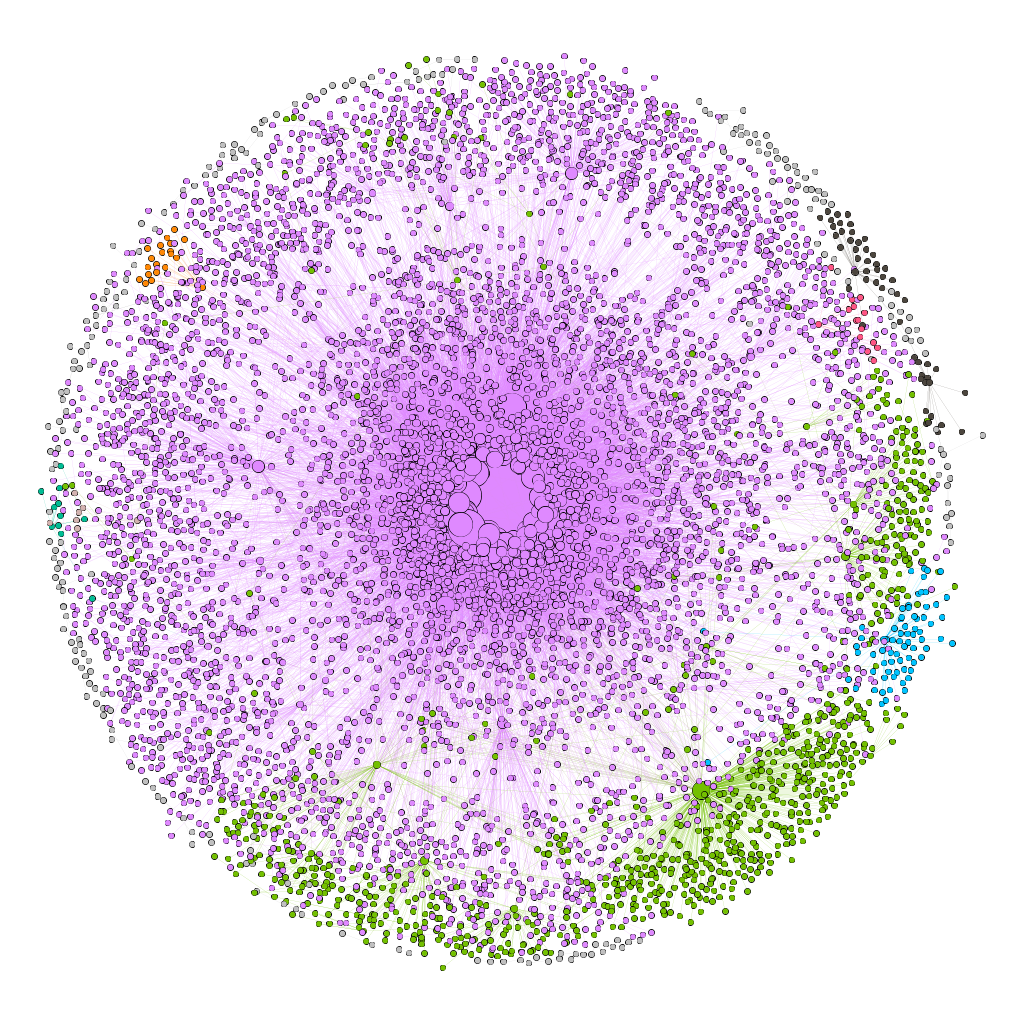
\includegraphics[width=0.5\textwidth ]{BLFWhole.png}
        \label{fig:BLF_graph}
    }
    \subfloat[]{
        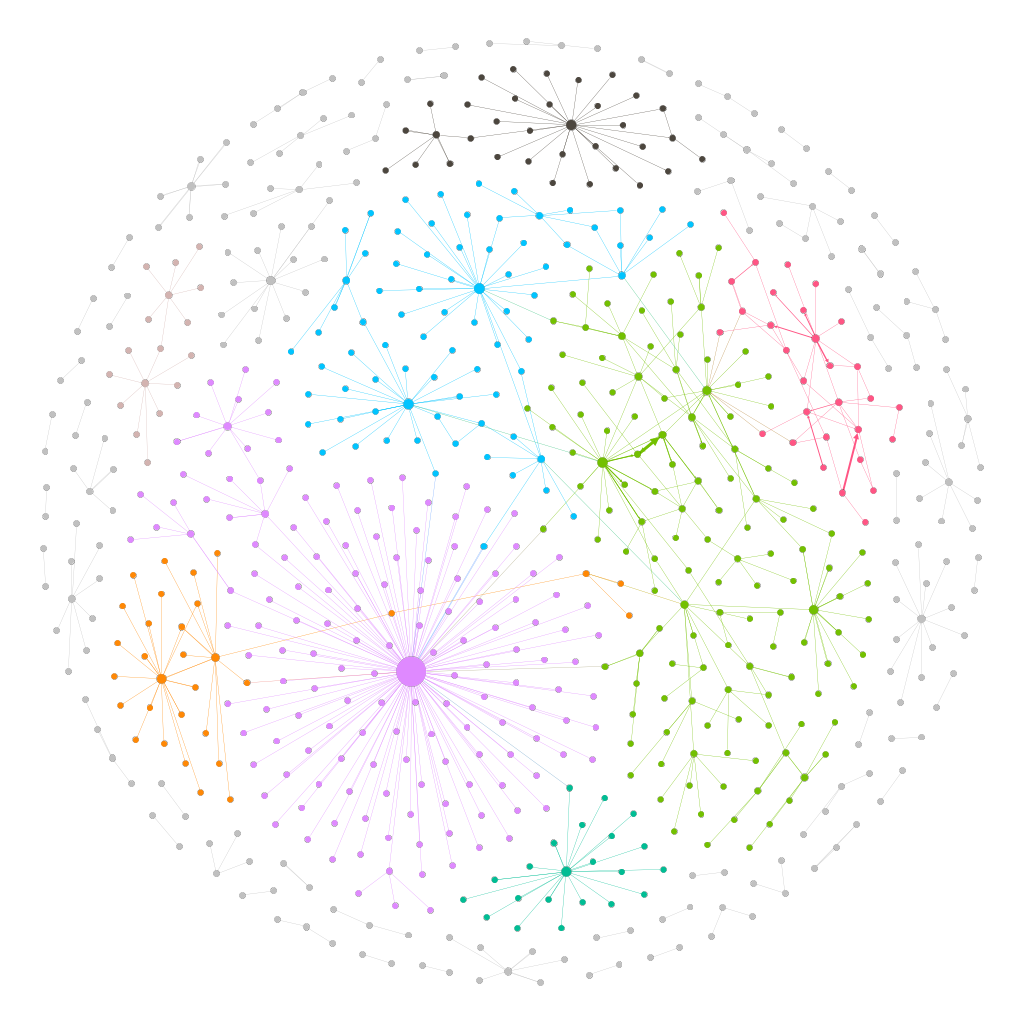
\includegraphics[width=0.5\linewidth ]{AsthamaWhole.png}
        \label{fig:Asthma_graph}
    }
    \caption{Global graphs prepared from Asthama UK community\ref{fig:Asthma_graph} and BLF community\ref{fig:BLF_graph}. The size of the node corresponds to the degree of the node and the color corresponds to the community membership }
\end{figure*}

These graphs abstractions ($G_g$ and $G_t$) represent the interaction structures which we intend to dissect. To understand the behaviour of these users, I evaluate several metrics on these graphs in order to understand the utility of these communities in terms of activity of sharing and support.

\subsubsection{Degree distributions and connectivity}
When you have a collection of nodes, connected to each other by edges, it is worth understanding how connected an average node is. More specifically, we would like to know the distribution of degrees, or the amount of edges a node has, across all the nodes in a graph. This metric is called the degree distribution of a graph, and it has been widely used in the complex networks literature as a measure to characterize types of graphs ~\cite{muchnik2013origins,ahn2007analysis,leskovec2008microscopic,raman2019challenges}.
We are specifically interested the nodes(users) who belong to the highest 1\% range of degrees. These users are the ones who are most interactive and have established edges with a lot of other users by exchanging messages. These users are called ``superusers''. 

\subsubsection{Largest connected component}
A largest connected component of a graph $G(V,E)$ )is the largest possible sub-graph $G_L(V_L,E_L)$ of $G$, such that each node in $G_L$ has at least one valid connected path to every other node in $G_L$. By evaluating the largest connected component on $G_g$, we can find the subset of users in the community which form a cohesive community. Furthermore, by measuring the effect of removal of certain ``superusers'' from this sub-graph on the overall size and structure on $G_L$, once can deduce the importance of the said users to the cohesiveness of a community. 
We can also measure the characteristics of the largest component on a temporal basis. By examining the fraction of users in a given week that belong to the largest connected component, one can estimate the focused and cohesive nature of interactions.


\subsubsection{Social capital and triadic closure} According to the literature, social capital is defined as those features of social structures, such as interpersonal trust and norms of reciprocity and mutual aid, which act as resources for individuals and facilitate collective action~\cite{collins1993social,coleman1988social}
It is common to quantify social capital in the context of social networks, by looking at structural holes, or unmet potential social links in the network. This is where ties between otherwise unconnected neighbours are filled in, sometimes called as closures, thereby benefiting the broker and the two neighbours by adding an extra link for information to diffuse. 
Such mechanisms have been studied in the sociology literature for decades. Work by Granovetter~\cite{granovetter1977strength} explored these structural holes and proposed that they are detrimental for efficient diffusion of information and resources in social networks. He also at times called these the ``forbidden triad'', referring to their propensity to close up in social networks. Such closures are, according to Ronald Burt~\cite{burt2004structural,burt2009structural}, necessary for information brokerage, and at times directly equate to social capital of these broker nodes.
In our case, as so much evidence has shown that the brokers of social support are often the superusers, we would certainly want to investigate how these users affect the cohesion and structural holes in the graph.


\section{How do support communities thrive ?}
To answer the \textbf{RQ1}, it is first worth asking how the user interactions bind the community together. We would like to know if the messaging activity is highly concentrated around a few sets of users or is it covering a large fraction of the user base. More so, it is worth asking if there are any special users who bear the mantle of providing support. This can be observed from the measured metrics of the interaction graph. 
From table\ref{table:jmirData}, it is evident that a minority of users are generating a bulk of data on these communities. E.g. the top 1\% users by activity contributed 32\% posts to AsthamaUK community. Such level of activity makes these users extremely important in understanding the dynamics of support on these communities. We term these users as ``Superusers''.
But before looking at the role of these superusers, it is first worth analysing the overall activity patterns on these communities. Do these communities drive enough engagement and activity to sustain them over long periods of time?  

\subsection{Temporal activity patterns}
\label{sec:activity}
\begin{figure}[!ht]
    \centering
    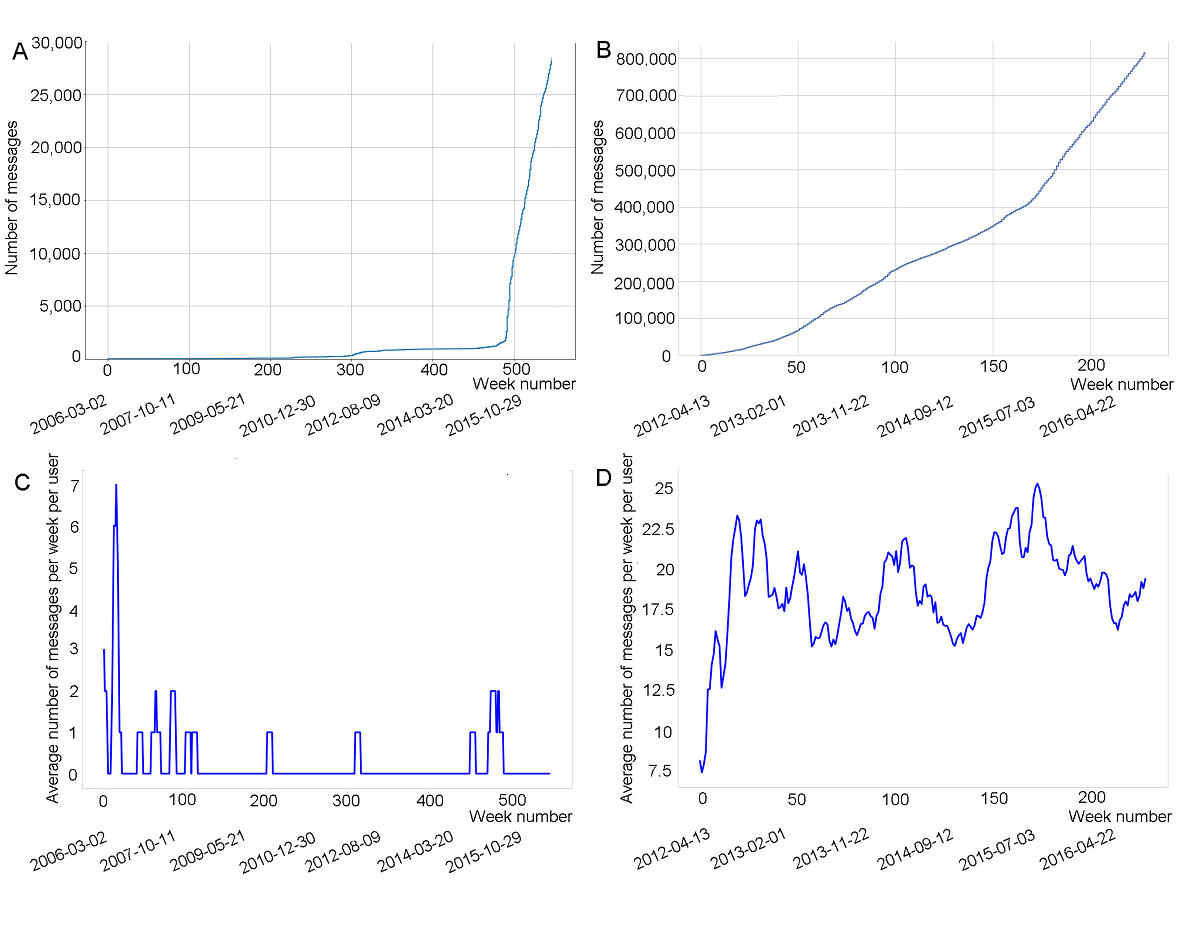
\includegraphics[width=\textwidth ]{Activity.png}
    \caption{Cumulative distributions of the number of posts as a function of time (weeks) within the Asthma UK (A) and the British Lung Foundation (B) communities. Calendars dates are reported below as week numbers (since the inception of the community). Panels C and D illustrate the average number of posts per user per week within Asthma UK and British Lung Foundation, respectively}        \label{fig:activity}
\end{figure}
To calculate the activity patterns of users on these forum, we first work with the most basic of proxies, which is the weekly/daily activity. We arrive at it by calculating the amount of messages exchanged in a community across the whole life cycle of the data. This metric would expose how much activity is happening on a daily or weekly basis on a particular community. It is worth noting that this activity pattern would also shed light on how users are engaging with the community. A continuous engagement is good for the vitality of a community, however if a community revolves around purely functional interactions, you may see a bursty nature of user activity across time~\cite{panzarasa2015emergence}. 

Figure ~\ref{fig:activity} shows the activity patterns on both the health communities on a cumulative and weekly basis. It was quite evident that the BLF community was more active of the two, in that, the community exhibits a consistent engagement by the users across the lifetime of the data as well as on a weekly basis. The Asthma forum however shows a bursty nature, despite being more than twice as old as the BLF community. One possible explanation can arise from the nature of these two illnesses. Asthma tends to be an episodic disease, with flare-ups in patients happening from time to time. These flare-ups are also often seasonal in nature, happening in sync with the pollen cycles in the air~\cite{dellavalle2012effects}. On the contrary, the British Lung Foundation forum deals with, alongside Asthma, diseases that are chronic in nature such as Chronic Obstructive Pulmonary Disorder (COPD) and Emphysema. This means these patients are constantly activated and tend to engage with the community on a more frequent basis. 

\subsection{Cohesive conversations}

\begin{figure}[!ht]
    \centering
    % \hspace*{-5mm}
    \subfloat[]{
        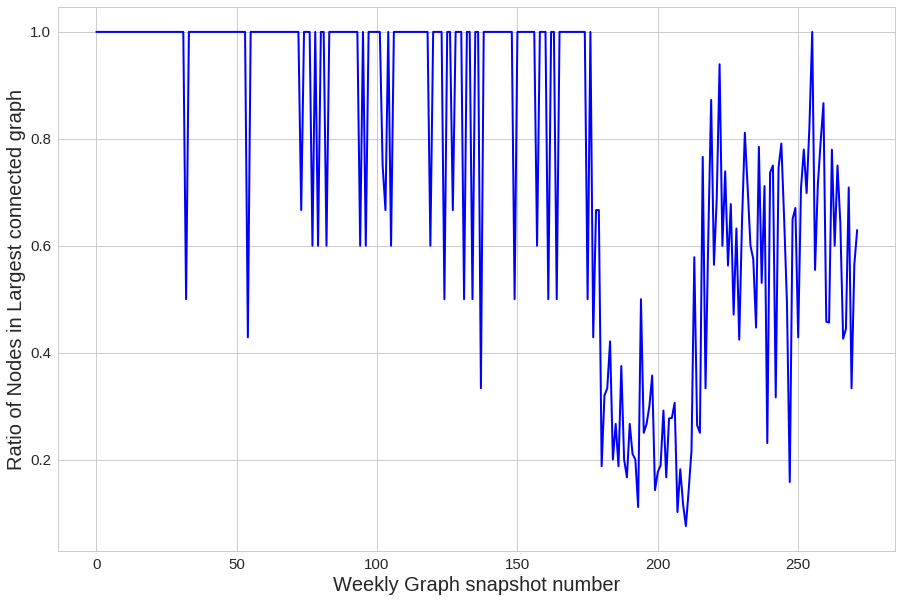
\includegraphics[width=0.5\textwidth ]{ConnectedComponent_weekly_ashtma.png}
        \label{fig:lcc_asthma}
    }
    \subfloat[]{
        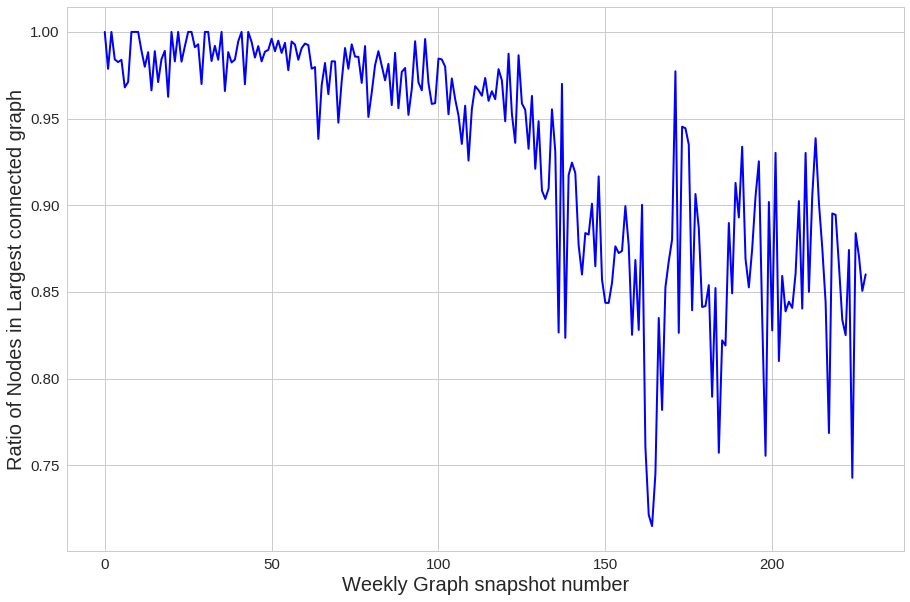
\includegraphics[width=0.5\linewidth ]{weekly_largest_component_BLF.png}
        \label{fig:lcc_blf}
    }
    
    \caption{Fraction of users that are part of the largest component as a function of time (weeks) for Asthma UK \ref{fig:lcc_asthma} and the British Lung Foundation \ref{fig:lcc_blf}.}
\end{figure}

To understand the first aspect of the community's resilience, I examine how is the coverage of communications between the users, on a weekly basis, given that messages are exchanged between the most active users within that week. 
To do so, imagine a sorted list of message interactions over a particular time period $T_k$, sorted in chronological order defined as $L_k=[E_{ij} \forall i,j \in N]$ , where $E_{ij}$ is a message between user $i$ and user $j$, with $N$ total users being active in a given time period $T_k$. Now imagine this time period $T_k$ is of 7 days . I calculate such $K$ lists for the $K$ weeks the community has been active. For each such list, I induce a graph $G_k(V,E)$ such that the nodes in $V$ are the active users in that particular list, and the edges in $E$ are corresponding to the messages exchanged in the list $L_k$ between any two users. 
Now for each such graph $G_k$ I calculate the largest connected subgraph $G_{\theta_k}(N_k,E_k)$ such that all nodes in $N_k$ have at least one path between them. Calculating the fraction $\frac{N_k}{N}$ would give us the total fraction of users who are part of the same conversation network for a given week. After calculating and plotting these fractions across a total of 250 weeks for each community, we see that whenever there is an activity on these networks, almost always, the active nodes belong to the largest connected sub graph. This implies that activity on support forums is cohesive and even if bursty at times, is all encompassing with the users. 

It is worth noting that as the activity on the communities increases, you see an increase in fragmentation of the graph structure with the ration of nodes in the Largest component dropping considerably(See figure \ref{fig:lcc_asthma} and \ref{fig:lcc_blf}). Which means there are concurrent discussions  happening with disjoint set of users. 



\subsection{Fragile global structure}
\label{sec:fragility}
\begin{figure}[!ht]
    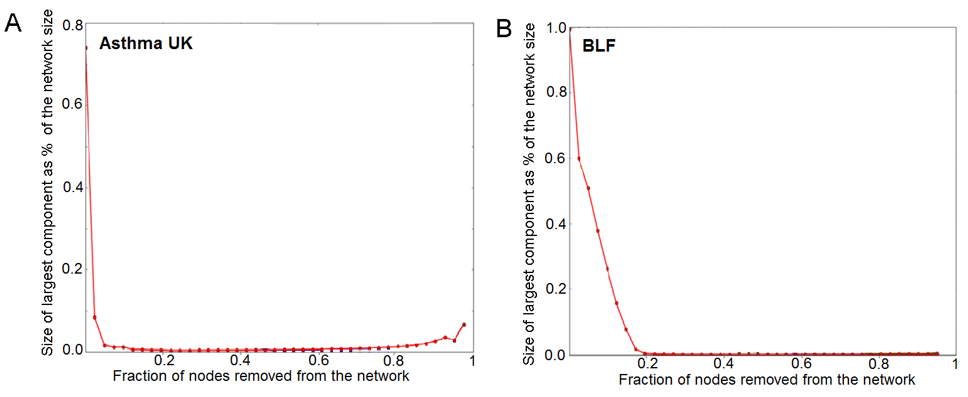
\includegraphics[width=\textwidth]{jmirSensitivity.png}
    \caption{Results of progressive removal of superusers. Both communities collapse drastically, in terms of connectivity, with BLF showing a marginally more resilience }
    \label{fig:sense_asthma}
\end{figure}
Despite the exchange on a weekly basis is quite cohesive, it is pertinent to understand the resilience in terms of user responsibility in helping, in order to examine the health of such a community. Moreover, I want to know if the conversation network is held together by a more or less uniform contribution of nodes, or if there is a skew in the responsibility of nodes. 
This can be tested by using the sensitivity analysis methods, popular in the network science~\cite{braunstein2016network,albert2000error}, which measures the network's capacity to diffuse information as you remove nodes based on certain property. In our case, we want to understand the importance of the \textsl{Superusers}, or the users who are disproportionately more active. Hence we begin by first sorting all the nodes in the macroscopic graph $G(V,E)$ in order of their degrees. The degree of a node in the global graph is proportional to the diverse set of users that node has communicated with, over the period if the community's lifetime. We then start removing nodes from the top, by progressively removing nodes in increments of 1\%. I then compute the size of the largest connected component $G_k$ and compute the ration of number of nodes in $G_k$ as compared to the original global undisturbed network.  Figure \ref{fig:sense_asthma} shows the performance of global graphs of both the communities to this attack. It is worth noting, that what we observe is that a top 10\% nodes by activity are responsible for most of the cohesive connectivity of the community. This also means that the top 10\% of these nodes have the most diverse connections in terms of number of users contacted. This gives hope to health care industry, since these nodes can act like efficient information diffusers, if used in a targeted fashion. 

\subsection{Anti-rich conversations}
\label{sec:richclub}
\begin{figure}[!ht]
    \centering
    % \hspace*{-5mm}
    \subfloat[]{
        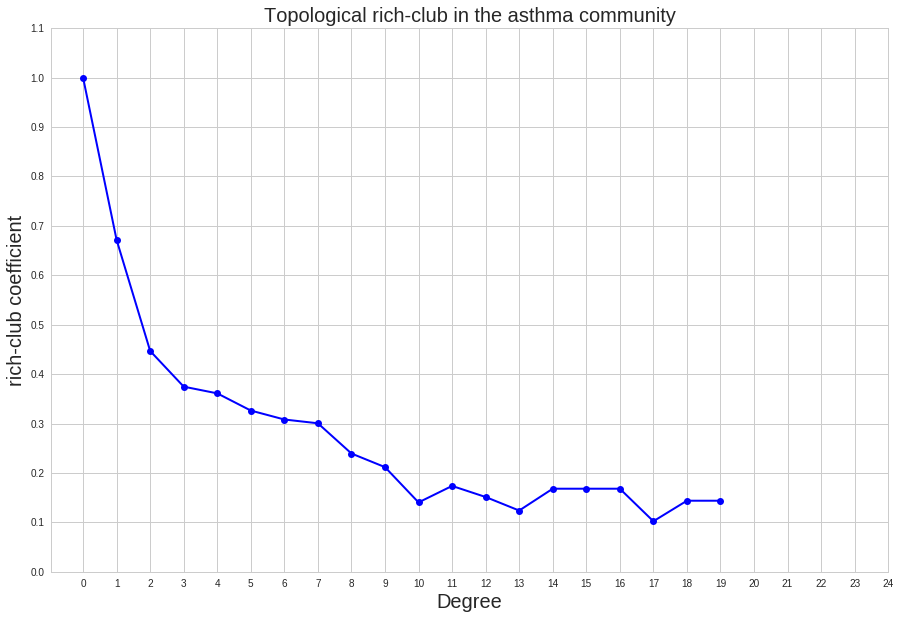
\includegraphics[width=0.5\textwidth ]{RichClub_asthma_truncated.png}
        \label{fig:rich_asthma}
    }
    \subfloat[]{
        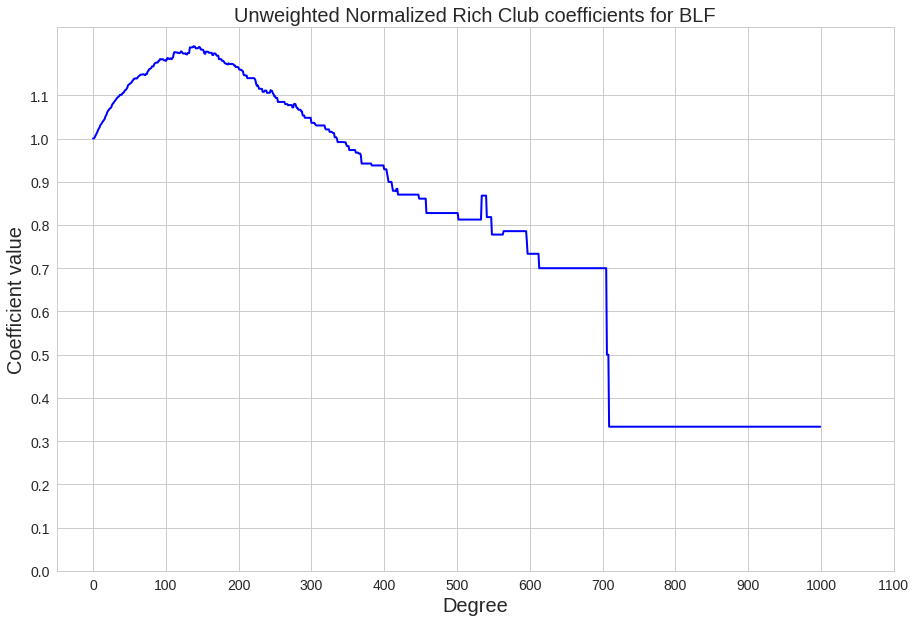
\includegraphics[width=0.5\linewidth ]{RichClub_BLF_truncated.png}
        \label{fig:rich_blf}
    }
    \caption{ Plots of rich-club coefficients for each viable degree in the respective communities. Both communities exhibit values less than 1, indicating an anti-rich behaviour by the well connected nodes.  }
\end{figure}
The “rich-club” coefficient is a metric designed to measure the extent to which well-connected users tend to connect with one another, to a higher degree than expected by chance~\cite{colizza2006detecting}. To this end, for each value k of a node’s degree (ie, the number of other users a given user is connected with), we computed the ratio between the number of actual connections between nodes with degree k or larger and the total possible number of such connections~\cite{opsahl2008prominence}. We then divided this ratio by the one obtained on a corresponding random network with the same number of nodes and degree distribution (ie, the probability distribution of the degrees over the whole network) as the real network, but in which links were randomly reshuffled between nodes. 

Formally let $G(V,E)$ be a global graph representation of the community. Let $V_{>k}$ be the set of vertices in the graph having degree higher than $k$. Let there be $N_{>k}$ such vertices having $E_{>k}$ edges between them. In such case, the rich club coefficient for degree $k$ in the graph $G$ is given by 
\begin{equation}
 \phi(k) = \frac{2E_{>k}}{N_{>k}(N_{>k} - 1)}
 \label{eq:rich_club}
\end{equation}
In this equation $\frac{N_{>k}(N_{>k} - 1)}{2}$ represents the maximum number of edges possible between $N_{>k}$ nodes. These coefficients are highly dependent on the size of the network, which makes them hard to compare. So I normalize the network by comparing against a random null model of rich-club coefficients $\phi_{rand}(k)$. This is obtained by generating an ensemble of random networks, each having the same degree distribution as that of $G$, but with links randomly placed. The ratio $\frac{\phi(k)}{\phi_{rand}(k)}$, gives us an un-correlated trend about the rich-club effect in $G$. 

Thus, the rich-club coefficients may take values lower or higher than 1, depending on whether the real network has a higher or lower tendency to coalesce into rich clubs than randomly expected. In particular, networks that display a high rich-club coefficient (ie, greater than 1, are also said to show a “rich-club effect,” namely the tendency to organise into a hierarchical structure in which highly connected nodes preferentially create tightly knit groups with one another ~\cite{mcauley2007rich}. .

In most previous studies the rich-club coefficient in the technical and real world networks exhibits values larger than 1 as the degree of a node goes up. This shows a propensity to create rich-clubs, with highly connected nodes preferentially connecting with other highly connected nodes. Thus these networks exhibit exclusive clubs of (topologically) rich nodes, as illustrated in previous work~\cite{zhou2004rich,colizza2006detecting}. What we observe however in the cases of support communities is that in general we end up with a less than 1 rich-club co-efficient as the value of degrees $k$ goes up. This means, rich nodes are exhibiting an anti-rich behaviour, where nodes which have a higher degree prefer in engaging with new nodes with lower degree. This implies an active information exchange from a well connected node to a sparsely connected node, which we would expect in a supportive interaction according to the definition of social support.


\section{What differentiates \textbf{users} on support communities from generic ones?}
\label{sec:support}
Once we establish that these support communities are thriving and are providing what seems to be an active supportive environment for the users(anti-rich superusers), it is worth delving into the analytical methods for quantifying these supportive interactions. More so we would like to have concrete metrics that characterize a given community as a supportive one. To do so we need to understand how are the users on these communities driven to help each other, and whether there is a correlation between the ``richness'' of a user, as defined in previous section, and its propensity to help. More so we would like to know how consistent are these so called ``rich'' users in providing support. 

\subsection{Propensity to help} 
We would like to understand how users on support communities, as a group behave as they become more seasoned. Fortunately, there is an approximate way for us to capture a user's role as a support seeker and as a support giver. As described in Section \ref{sec:dataset}, the forum activity consists of a root poster, asking a question to the forum board, and the members responding to that question in a cascaded fashion. These responses, along with the original question constitute what is called as a \textsl{thread}.
To that end, we define the following two roles on these communities\footnote{There are other ways to qualify someone as support giver/seeker, mainly using language sturcture, but here we consider only the bare minimum requirement to be considered as one, using the position in conversation structure}

In the context for support forums, a support seeker is a user who begins a thread by posting on the forum, a question, or a query, to which others may respond to. Similarly a support giver is a user who responds to any post by a support seeker.

With this in mind, I aim to model the behaviour if users on these support communities in terms of being a support giver or a support seeker.

We first begin by calculating the average number of questions per user and answers per user across the dataset, by finding the mean number of questions and answers posted by any user on the forum. 
We consider an expected probability of answering a question by a user as $P_a$ as 2/3 and the probability of posting a question as $P_q$ as 1/3. 
With this information we modify the definition of ``Z-score'' to quantify the expertise, used by Adamic. et. al ~\cite{zhang2007expertise} to arrive at the expression of expertise in the context out our support community. 

 A user has two possible actions at any given time, while interacting with the community. They can either post a question on the forum, or answer to existing questions. The probability of doing either actions are $P_a$ and $P_q$ respectively. To that end, we try to model this interaction process as a Bernoulli process with two outcomes, having asymmetric probabilities. 
 
\begin{proof}
   
    Consider a Bernoulli process for a user to choose to answer or post a question on the forum, with asymmetric probabilities for answering ($P_a$) and posting a question ($P_q$). 
    For any user $i$ the total number of posts $n_i$ are the sum of total number of questions posted $q_i$ and answers posted $a_i$ and $n_i = a_i + q_i$
    For a Bernoulli process the variance for the whole forum is given as: 
     $$\sigma_{forum} = \sqrt{nP_a(1-P_a)}$$     $$\sigma_{forum} = \frac{\sqrt{2n}}{3}$$
    Similarly the mean for this process can be written as : 
    $$ \mu_{forum} = nP_a = \frac{2n}{3} $$
    $Z_{score}$ of a random variable $X$ is defined as 
    $$Z_{score} = \frac{X - \mu}{\sigma}$$
    Substituting the values for $\sigma_{forum}$ and  $\mu_{forum}$ inside the expression for $Z_{score}$ we arrive at the modified Z-score as 
    \begin{equation}
        Z_{score} = \frac{a-2q}{\sqrt{2(a+q)}}
    \label{eq:zscore}
    \end{equation}    
\end{proof}
Equation \ref{eq:zscore} depicts the modified notion of Z-score for the question answering process of our support community. I calculate this particular metric for each user in both the communities based on their posting history. 
\begin{figure}[!ht]
    \centering
    % \hspace*{-5mm}
    \subfloat[]{
        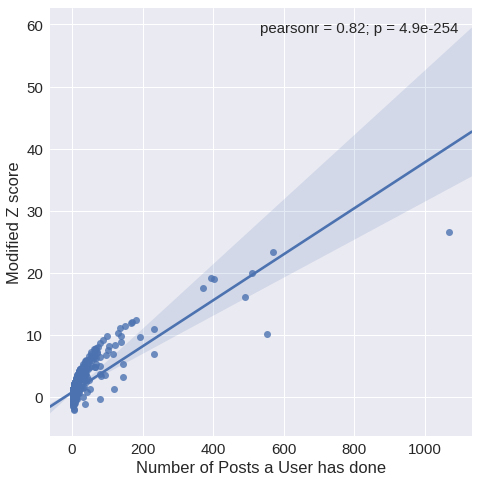
\includegraphics[width=0.5\textwidth ]{ModifiedZScore_asthma.png}
        \label{fig:zscore_asthma}
    }
    \subfloat[]{
        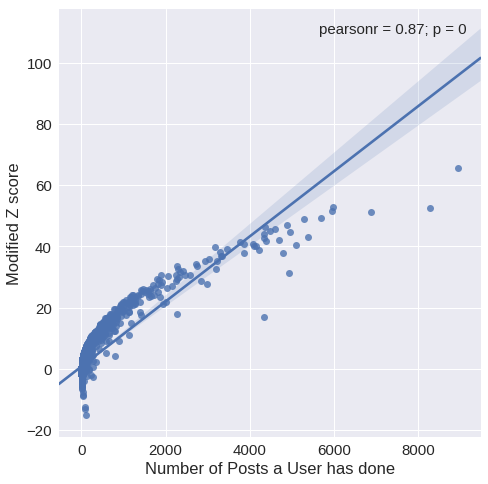
\includegraphics[width=0.5\linewidth ]{Modified_ZScore.png}
        \label{fig:zscore_blf}
    }
    \caption{  }
\end{figure}

I then find the correlation between a users Z-score and the total number of posts a user has done in their lifetime on the forum. Figure \ref{fig:zscore_asthma} and Figure \ref{fig:zscore_blf} shows the results of this analysis for both the communities. It is quite evident, that as the users become more seasoned and post more actively, they are more likely to answer on questions rather than post new ones. This also implies that based on the rich club results from Section \ref{sec:richclub}, these communities are thriving not only for the ``rich'' users, but also for the sparse users. Users on these communities are more open to new members and provide active support to them. 
Developing metrics like this makes quantifying whether a particular community works for the subscribers a tractable problem.


\subsection{ Superusers and structural holes }
One of the key aspects of utility of any social network is driven from the social capital offered as a result of the subscription. 


Till now we looked at the global macro structural properties of this support graph using the global graphs $G_g$, where we look at the user's interactions with other users across the lifetime of the community. But often the supportive interactions happen in a lifetime of a single thread, revolving around a topic or query. So to examine the effect of the superusers on the social cohesion, we correlate the total number of posts done by super users on any given thread, to the amount of closed triangles found in the corresponding thread graph $G_t$.  

\begin{figure*}[!ht]
    \centering
    % \hspace*{-5mm}
    \subfloat[]{
        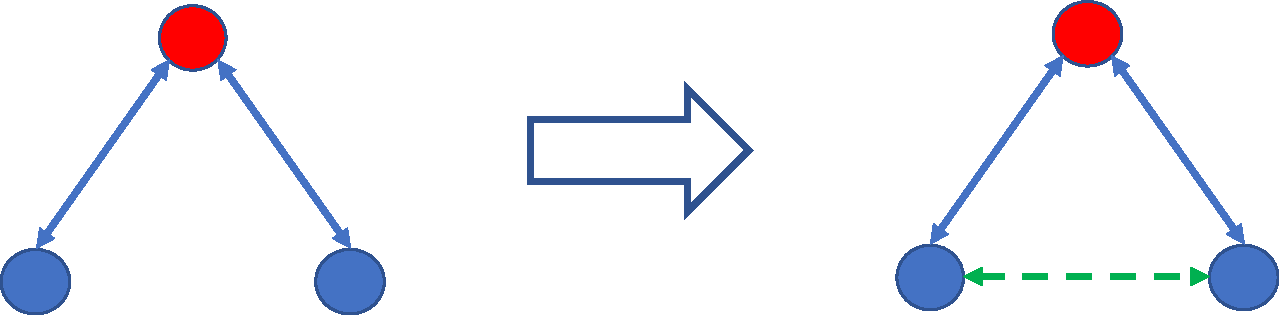
\includegraphics[width=\linewidth]{Closure.pdf}
        \label{fig:closure}
    }

    \subfloat[]{
        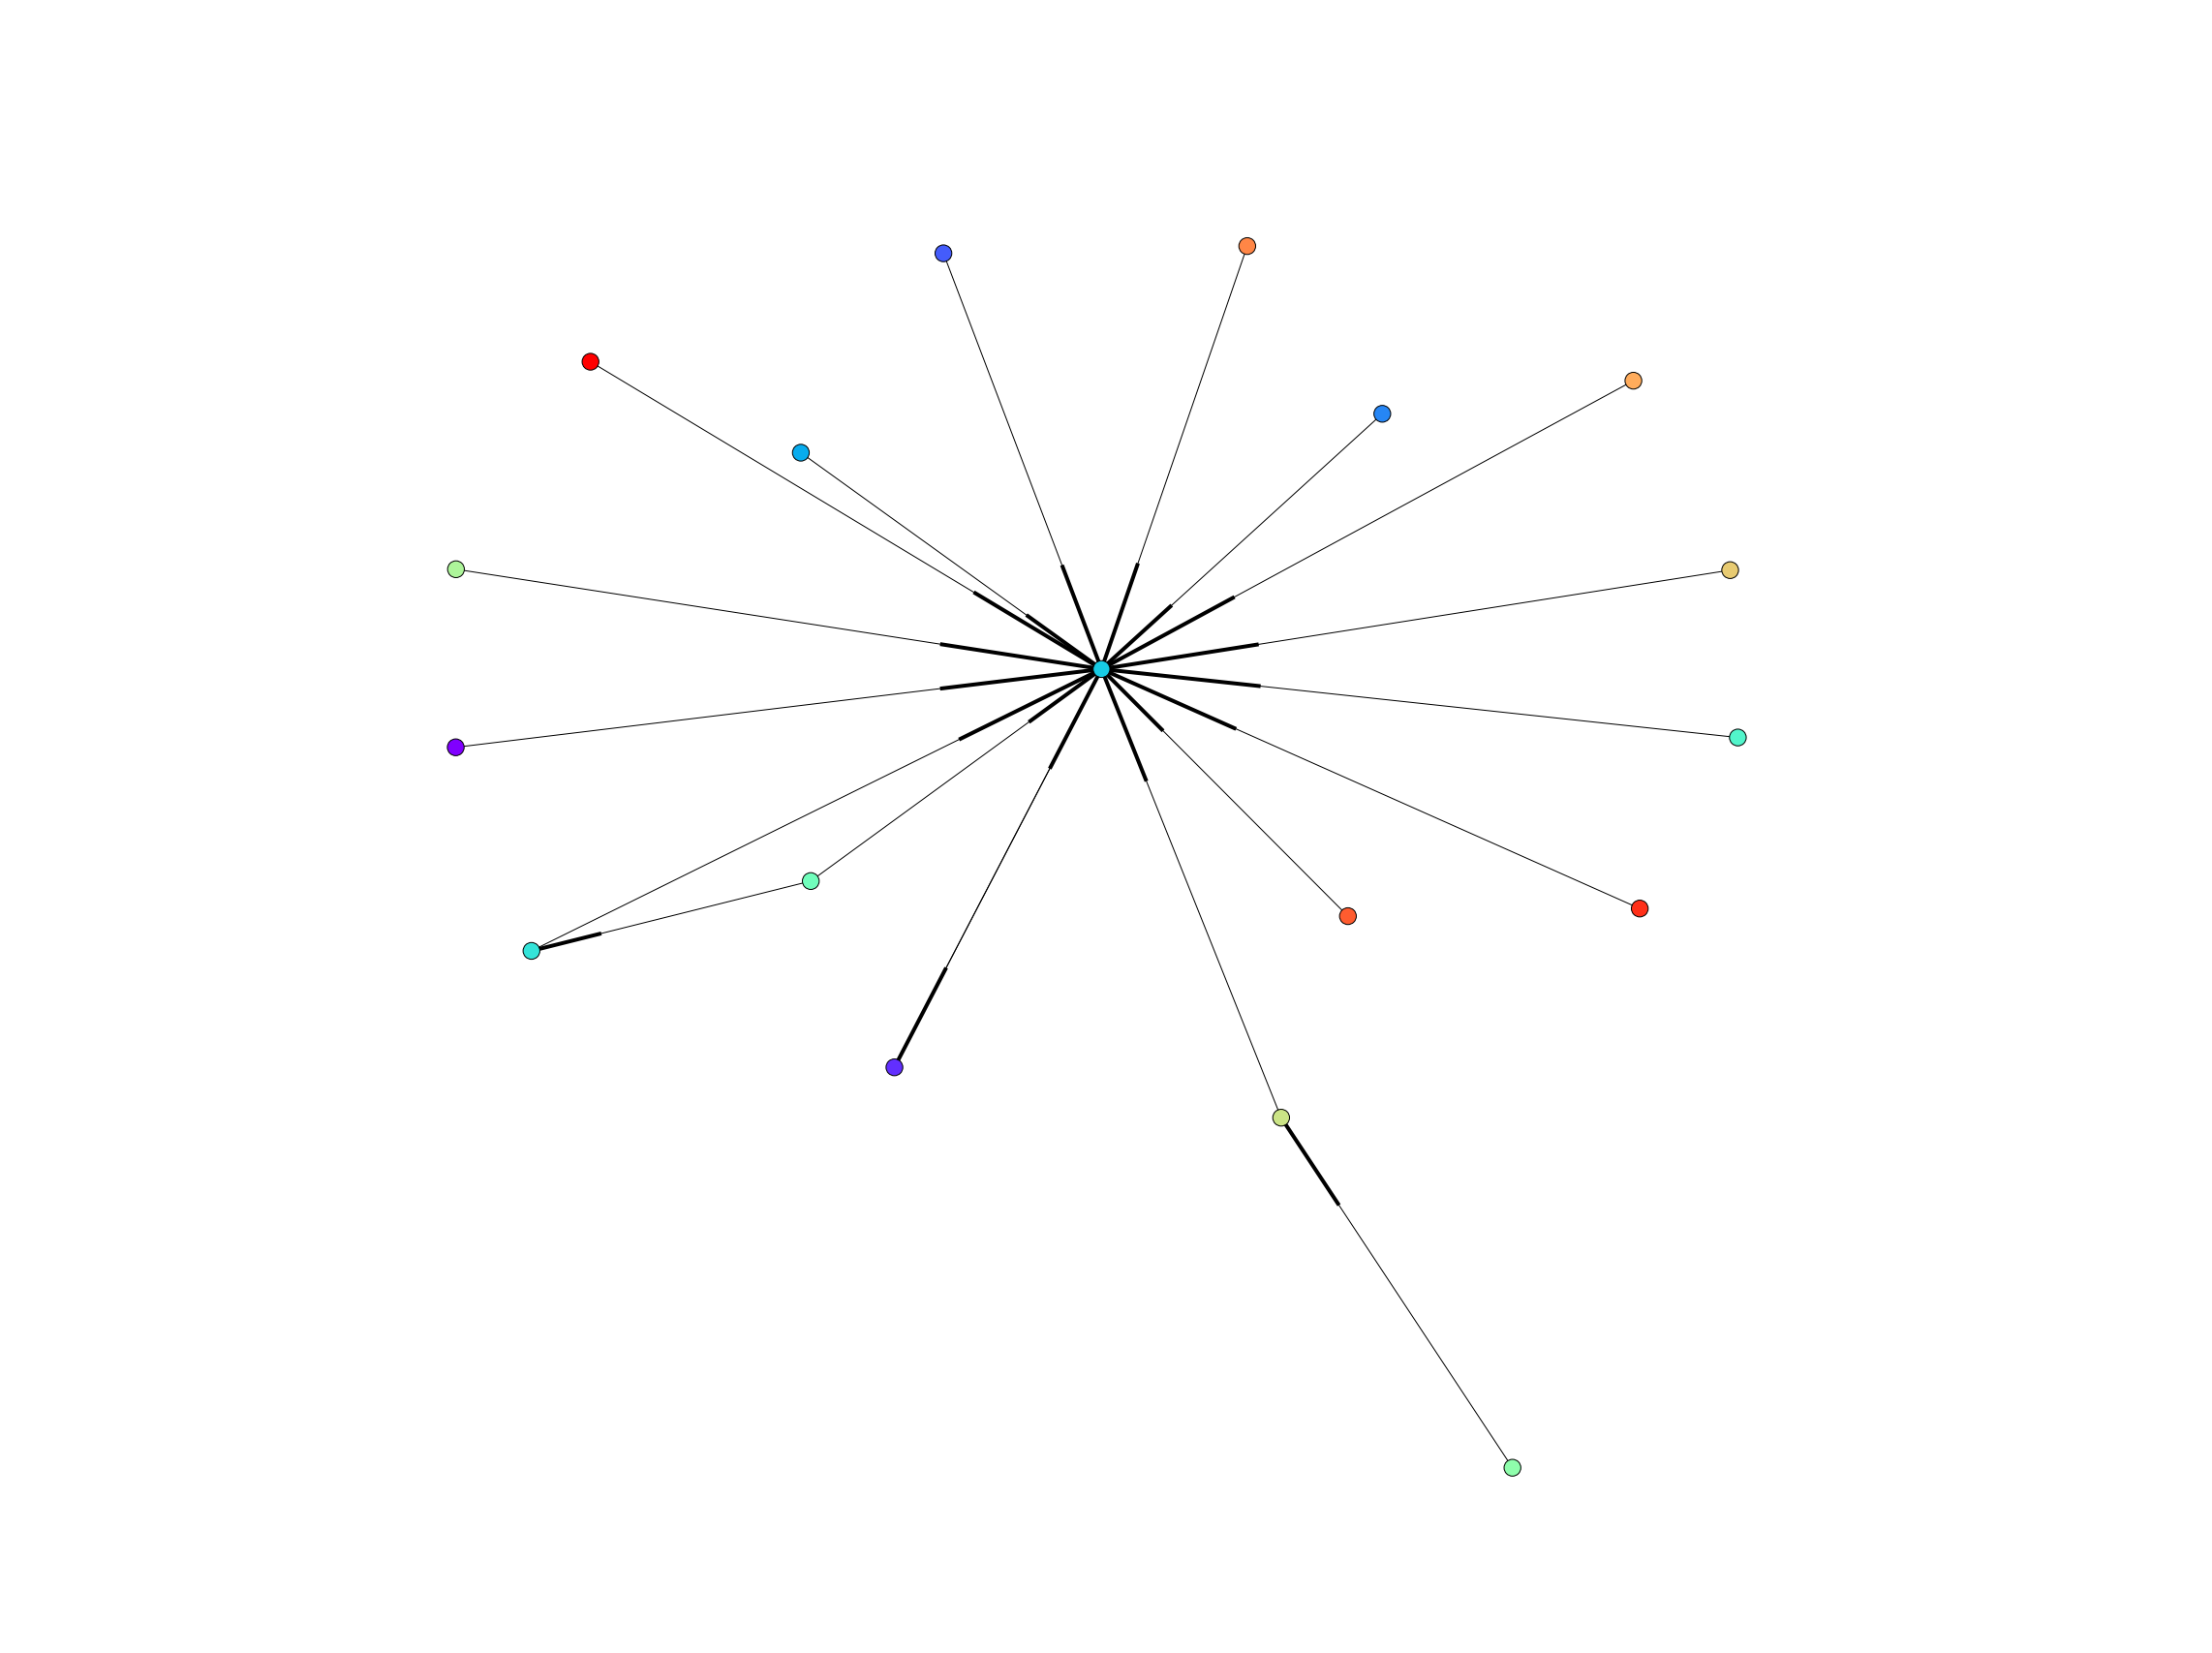
\includegraphics[width=0.5\linewidth ]{LowOPActivityGraph.png}
        \label{fig:noTri_op}
    }
    \subfloat[]{
    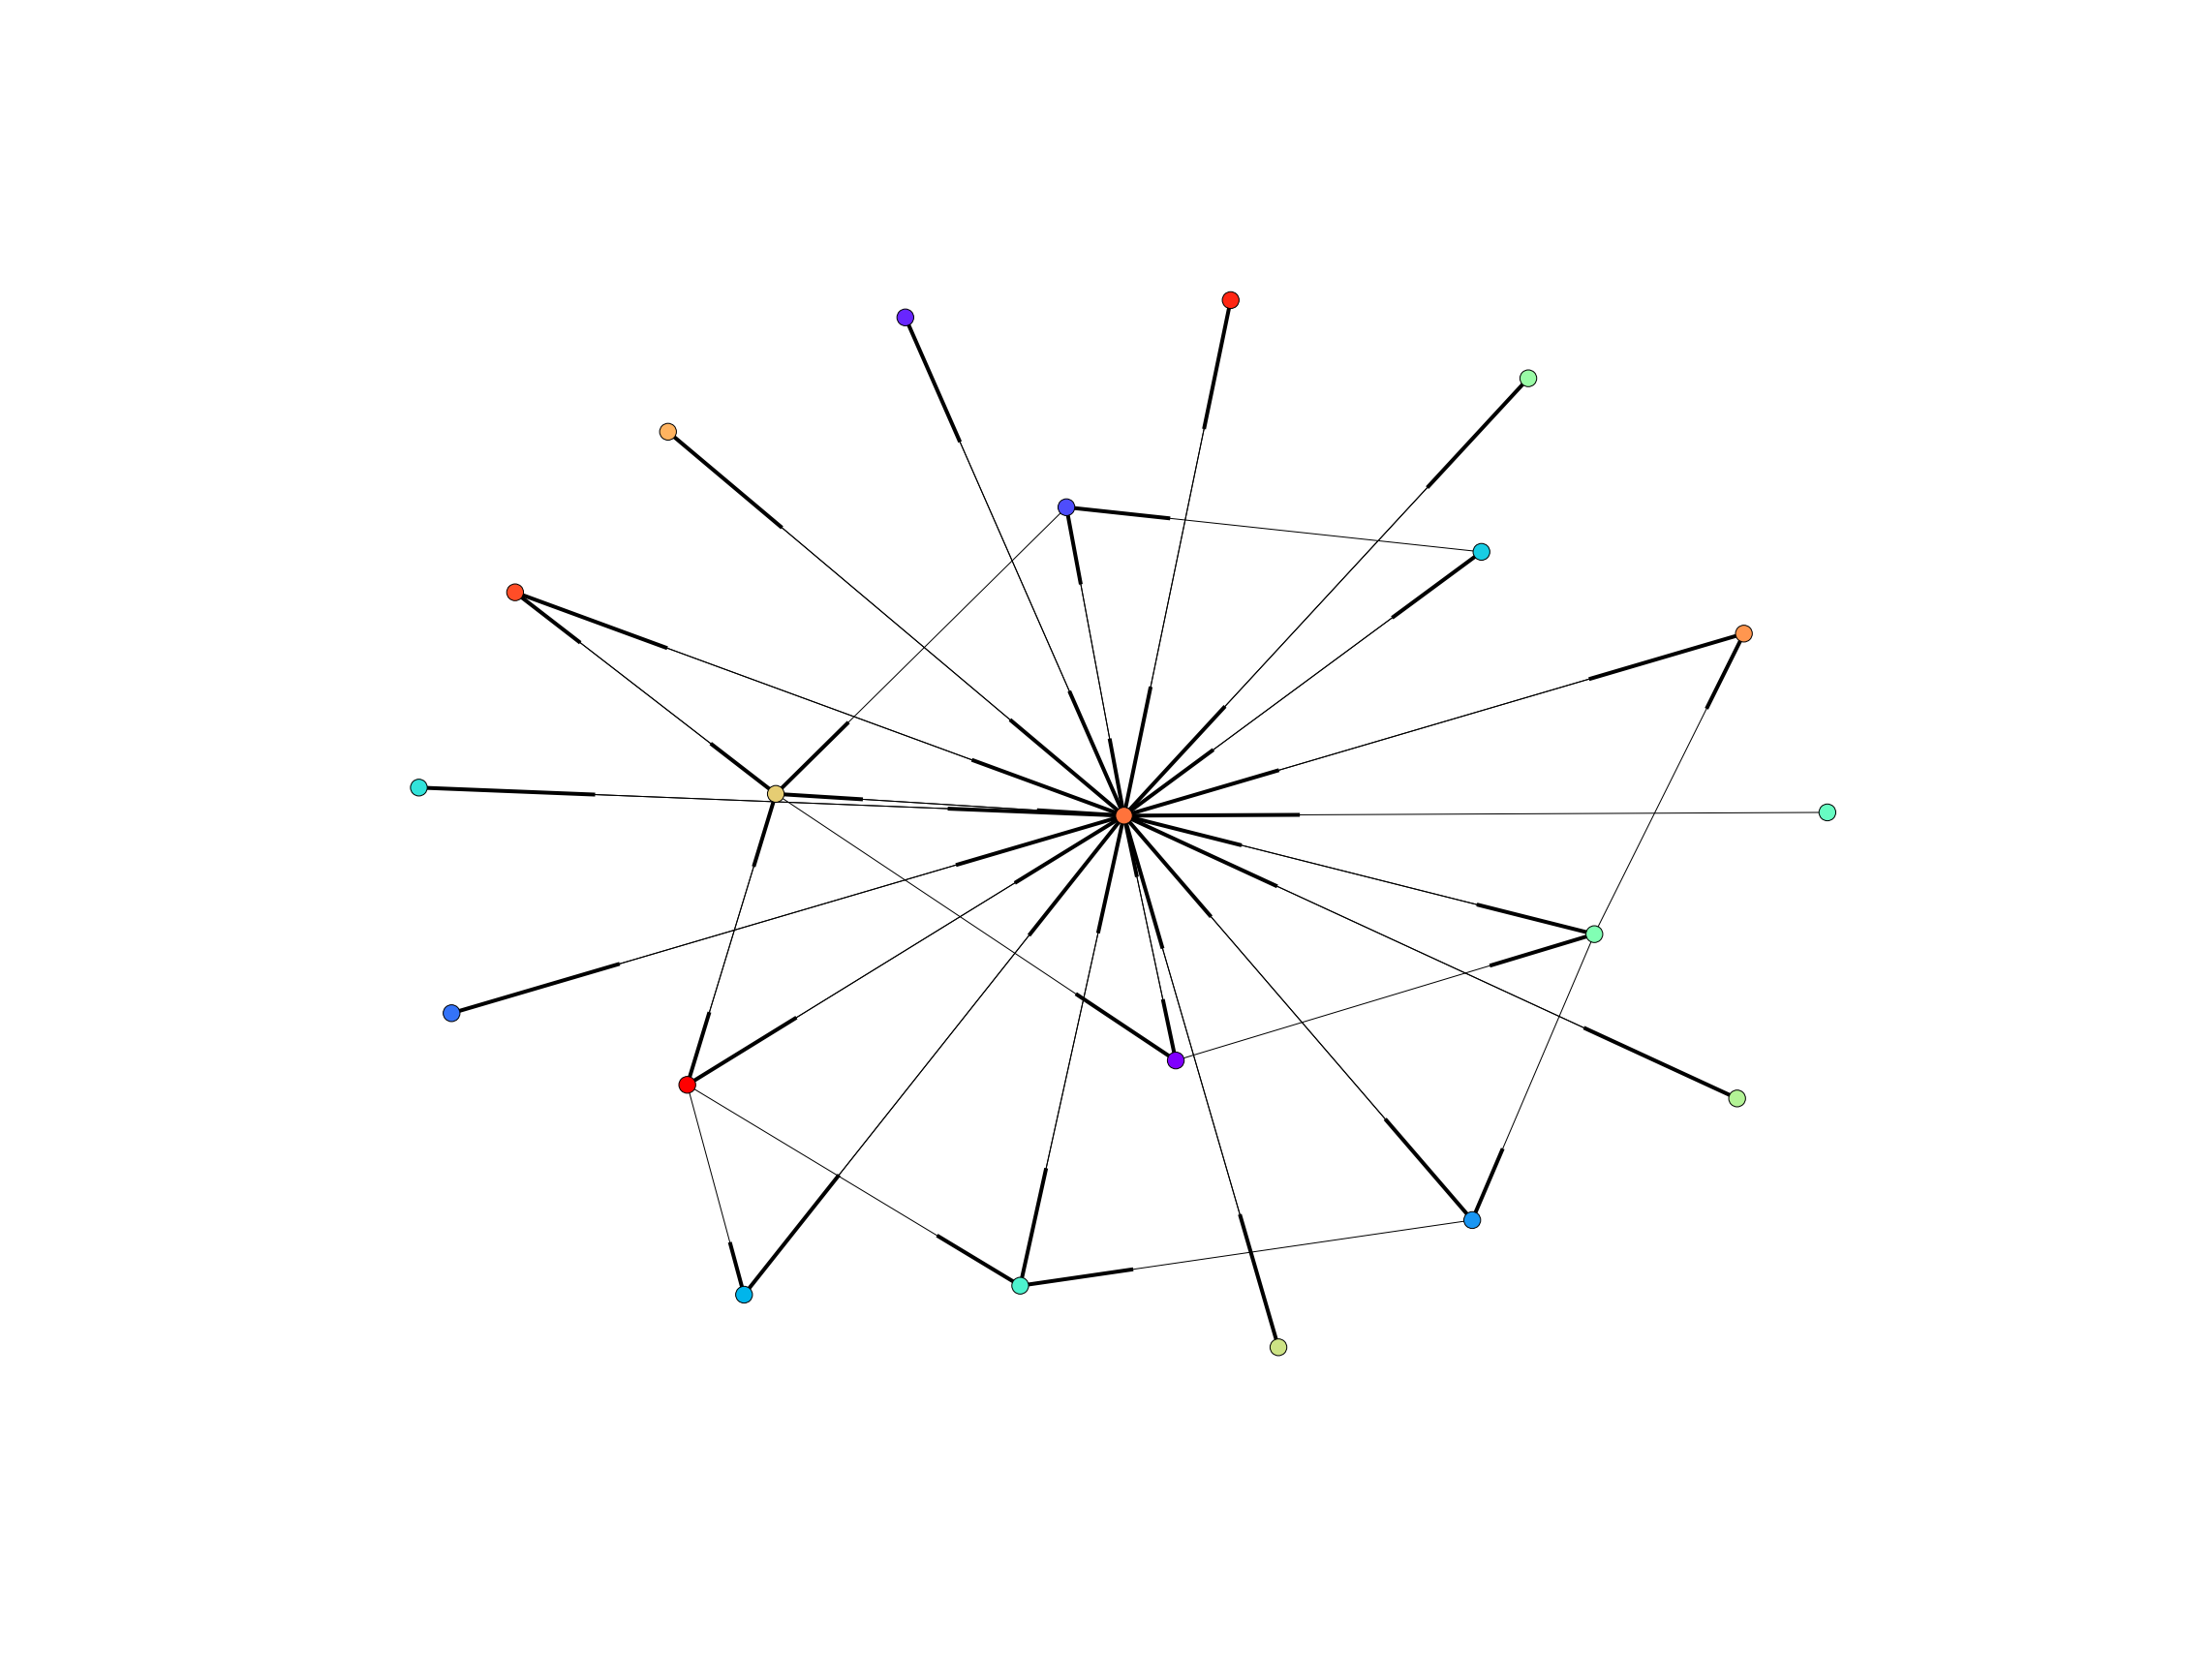
\includegraphics[width=0.5\linewidth ]{HighOPActivityGraph.png}
    \label{fig:Tri_op}
    }
    \caption{ Figure~\ref{fig:closure} shows an example of closure among three nodes, where a structural hole between a cluster of three nodes is closed by addition of the green link. Figure~\ref{fig:noTri_op} shows a thread level interaction graph showing lots of structural holes between participating nodes. On the other hand Figure~\ref{fig:Tri_op} shows an example of a thread level interaction graph where a `rich' user has contributed multiple times. This graph also shows more closures }
\end{figure*}

The resultant scatter plot can be seen in Figure~\ref{fig:TriCorr}, where we can see a net positive correlation of 0.44, with a very low p-value. This means there is a general trend of higher triadic closures in a conversation, with the amount of rich user participation.
 
\begin{figure}[!ht]
\centering
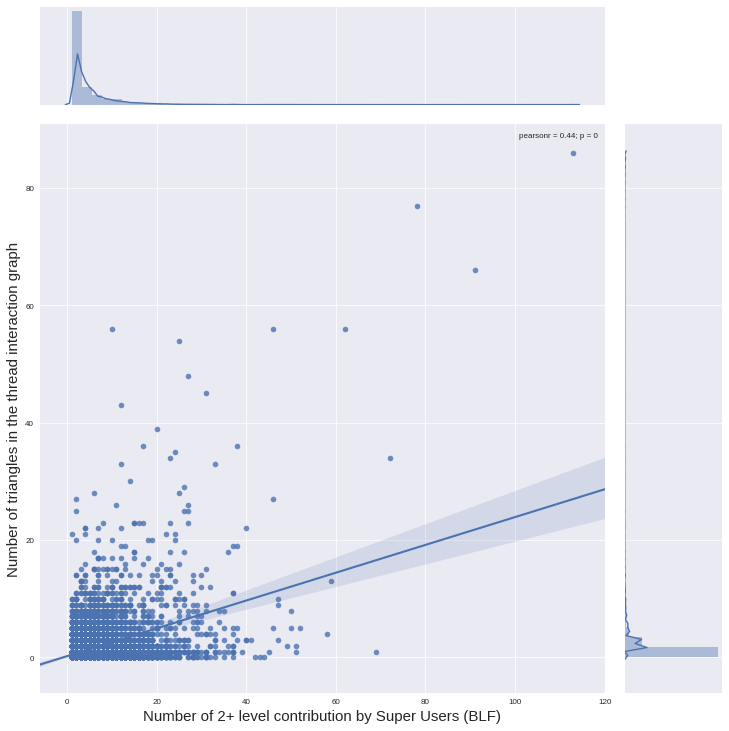
\includegraphics[width=0.7\linewidth ]{SUParticipationTriangles.png}

\caption{Scatter plot between the number of closed triangles in a conversation thread, with the total number of posts done by a superuser in that thread. A positive correlation of 0.44, with a p-value of 0 is observed. This indicates that the presence of a super user in a thread improves the over all cohesion of that thread and closes structural holes}
\label{fig:TriCorr}
\end{figure}

\section{Discussion}
In this chapter, we found that support communities show peculiar temporal and interaction dynamics. \textbf{RQ1} asked about the dynamics of support communities. We find that support communities exhibit a high level of engagement and participation. The communities are held together by the superusers. The removal of these superusers, collapses the network structure of these communities. \textbf{RQ2} asked about differentiating properties of users on support communities. We find that the users exhibit an anti-rich behaviour. This means that the superusers are engaging with less active users and are practising inclusion. We also find that users on support communities progress onto being support givers from support seekers with time. 
The idea of perceived support stems from the fact that the user in distress is not only getting the crucial information about the disease, but also benefits from the social capital of the allied users. We observe that  superusers tend to have a positive effect on the social capital of a conversation, promoting more social cohesion.

There is immense value in understanding how social support thrives on the internet, especially because of its potential to relieve the load off the ever so burdened health services. 
The work till now focussed on the global interactions of support givers and seekers on a community. It investigated the dynamics of support communities and looked at individual user's role in the larger scheme of things. 

In the next chapter, we would explore this problem from the scale of the entire conversation(macro) and from the scale of immediate local interactions in the ego network of a user(meso). This goes beyond looking at the individual actors of support, and quantifies the peculiar structure of a supportive conversation on the web.